\documentclass[letterpaper]{article} % DO NOT CHANGE THIS
\usepackage[submission]{aaai2027}  % DO NOT CHANGE THIS
% The serif, sans-serif, and monospaced fonts are loaded automatically by
% aaai2027.sty (newtxtext, helvet, courier). DO NOT add \usepackage{times},
% \usepackage{helvet}, \usepackage{courier}, or any other font package.
\usepackage[hyphens]{url}  % DO NOT CHANGE THIS
\usepackage{graphicx} % DO NOT CHANGE THIS
\urlstyle{rm} % DO NOT CHANGE THIS
\def\UrlFont{\rm}  % DO NOT CHANGE THIS
\usepackage{natbib}  % DO NOT CHANGE THIS AND DO NOT ADD ANY OPTIONS TO IT
\usepackage{caption} % DO NOT CHANGE THIS AND DO NOT ADD ANY OPTIONS TO IT
\frenchspacing  % DO NOT CHANGE THIS
%
% These are recommended to typeset algorithms but not required. See the subsubsection on algorithms. Remove them if you don't have algorithms in your paper.
\usepackage{algorithm}
\usepackage{algorithmic}

%
% These are recommended to typeset listings but not required. See the subsubsection on listing. Remove this block if you don't have listings in your paper.
\usepackage{newfloat}
\usepackage{multirow}
\usepackage{listings}
\DeclareCaptionStyle{ruled}{labelfont=normalfont,labelsep=colon,strut=off} % DO NOT CHANGE THIS
\lstset{%
	basicstyle={\footnotesize\ttfamily},% footnotesize acceptable for monospace
	numbers=left,numberstyle=\footnotesize,xleftmargin=2em,% show line numbers, remove this entire line if you don't want the numbers.
	aboveskip=0pt,belowskip=0pt,%
	showstringspaces=false,tabsize=2,breaklines=true}
\floatstyle{ruled}
\newfloat{listing}{tb}{lst}{}
\floatname{listing}{Listing}

%
% Required for aligned, substack, operatorname, etc.
\usepackage{amsmath}
% Recommended for better-looking tables
\usepackage{booktabs}

%
% Keep the \pdfinfo as shown here. There's no need
% for you to add the /Title and /Author tags.
\pdfinfo{
/TemplateVersion (2027.1)
}

% DISALLOWED PACKAGES
% \usepackage{authblk} -- This package is specifically forbidden
% \usepackage{balance} -- This package is specifically forbidden
% \usepackage{CJK} -- This package is specifically forbidden
% \usepackage{float} -- This package is specifically forbidden
% \usepackage{flushend} -- This package is specifically forbidden
% \usepackage{fullpage} -- This package is specifically forbidden
% \usepackage{geometry} -- This package is specifically forbidden
% \usepackage{hyperref} -- This package is specifically forbidden
% \usepackage{navigator} -- This package is specifically forbidden
% (or any other package that embeds links such as navigator or hyperref)
% \usepackage{indentfirst} -- This package is specifically forbidden
% \usepackage{layout} -- This package is specifically forbidden
% \usepackage{multicol} -- This package is specifically forbidden
% \usepackage{nameref} -- This package is specifically forbidden
% \usepackage{savetrees} -- This package is specifically forbidden
% \usepackage{setspace} -- This package is specifically forbidden
% \usepackage{stfloats} -- This package is specifically forbidden
% \usepackage{tabu} -- This package is specifically forbidden
% \usepackage{titlesec} -- This package is specifically forbidden
% \usepackage{tocbibind} -- This package is specifically forbidden
% \usepackage{ulem} -- This package is specifically forbidden
% \usepackage{wrapfig} -- This package is specifically forbidden
% DISALLOWED COMMANDS
% \nocopyright -- Your paper will not be published if you use this command
% \addtolength -- This command may not be used
% \balance -- This command may not be used
% \baselinestretch -- Your paper will not be published if you use this command
% \clearpage -- No page breaks of any kind may be used for the final version of your paper
% \columnsep -- This command may not be used
% \newpage -- No page breaks of any kind may be used for the final version of your paper
% \pagebreak -- No page breaks of any kind may be used for the final version of your paper
% \pagestyle -- This command may not be used
% \tiny -- This is not an acceptable font size.
% \vspace{- -- No negative value may be used in proximity of a caption, figure, table, section, subsection, subsubsection, or reference
% \vskip{- -- No negative value may be used to alter spacing above or below a caption, figure, table, section, subsection, subsubsection, or reference

\setcounter{secnumdepth}{0} %May be changed to 1 or 2 if section numbers are desired.

% The file aaai2027.sty is the style file for AAAI Press
% proceedings, working notes, and technical reports.
%

% Title

% Your title must be in mixed case, not sentence case.
% That means all verbs (including short verbs like be, is, using,and go),
% nouns, adverbs, adjectives should be capitalized, including both words in hyphenated terms, while
% articles, conjunctions, and prepositions are lower case unless they
% directly follow a colon or long dash
\title{From Compression Methods to Deployment Decisions: Quality-Constrained Fine-Grained Strategy Optimization for Efficient LLM Inference}
\author{
    %Authors
    % All authors must be in the same font size and format.
    Written by AAAI Press Staff\textsuperscript{\rm 1}\thanks{With help from the AAAI Publications Committee.}\\
    AAAI Style Contributions by Peter Patel Schneider,
    Sunil Issar,\\
    J. Scott Penberthy,
    George Ferguson,
    Hans Guesgen,
    Francisco Cruz\equalcontrib\corresponding,
    Marc Pujol-Gonzalez\equalcontrib\corresponding
}
\affiliations{
    %Afiliations
    \textsuperscript{\rm 1}Association for the Advancement of Artificial Intelligence\\
    % If you have multiple authors and multiple affiliations
    % use superscripts in text and roman font to identify them.
    % For example,

    % Sunil Issar\textsuperscript{\rm 2},
    % J. Scott Penberthy\textsuperscript{\rm 3},
    % George Ferguson\textsuperscript{\rm 4}\corresponding,
    % Hans Guesgen\textsuperscript{\rm 5}
    % Note that the comma should be placed after the superscript

    1101 Pennsylvania Ave, NW Suite 300\\
    Washington, DC 20004 USA\\
    % email address must be in roman text type, not monospace or sans serif
    proceedings-questions@aaai.org
%
% See more examples next
}

%Example, Single Author, ->> remove \iffalse,\fi and place them surrounding AAAI title to use it
\iffalse
\title{My Publication Title --- Single Author}
\author {
    Author Name
}
\affiliations{
    Affiliation\\
    Affiliation Line 2\\
    name@example.com
}
\fi

\iffalse
%Example, Multiple Authors, ->> remove \iffalse,\fi and place them surrounding AAAI title to use it
\title{My Publication Title --- Multiple Authors}
\author {
    % Authors
    First Author Name\textsuperscript{\rm 1,\rm 2}\equalcontrib,
    Second Author Name\textsuperscript{\rm 2}\equalcontrib,
    Third Author Name\textsuperscript{\rm 1}\corresponding
}
\affiliations {
    % Affiliations
    \textsuperscript{\rm 1}Affiliation 1\\
    \textsuperscript{\rm 2}Affiliation 2\\
    firstAuthor@affiliation1.com, secondAuthor@affilation2.com, thirdAuthor@affiliation1.com
}
\fi


\begin{document}

\maketitle

\begin{abstract}
% Model compression has become an effective approach for reducing the inference cost of large language models (LLMs). However, from the perspective of practical deployment, existing methods still leave two critical challenges unresolved: they lack a unified mechanism for selecting among different compression techniques, and they cannot automatically provide compression strategies with appropriate speed--quality trade-offs for diverse deployment requirements. In this work, we propose \textbf{DASO}, a deployment-oriented framework for heterogeneous LLM compression strategy optimization. It integrates quantization and pruning into a unified candidate space and automatically selects module-wise and inference-stage-wise configurations under a user-defined quality constraint. To enable efficient optimization, we develop a hardware-aware latency model with shape- and policy-level calibration, together with a structure-aware quality model that estimates global quality degradation from local compression perturbations. A constrained optimizer then selects module- and stage-wise compression strategies under the given quality budget, and the resulting strategies are finally deployed through an extended vLLM runtime. Experiments on Llama-2-7B-Chat and Llama-3.1-8B-Instruct on an RTX~5090 GPU demonstrate that our framework achieves \textbf{1.14$\times$--2.08$\times$} end-to-end speedups over the BF16 baseline across different quality budgets, delivering favorable speed--quality trade-offs across deployment scenarios.
Model compression has become an effective approach for speeding up large language model (LLM) inference. However, the availability of diverse compression methods does not directly translate into actionable deployment decisions: existing approaches lack a unified mechanism for selecting among compression techniques at a fine granularity---across model modules and across inference stages such as prefill and decode---and they cannot automatically generate strategies with appropriate speed--quality trade-offs for diverse deployment requirements. In this work, we propose \textbf{DASO} (Deployment-Aware Strategy Optimization), a deployment-oriented framework that turns a set of compression methods into fine-grained deployment decisions. DASO integrates quantization and pruning methods into a unified candidate space and automatically selects module-wise and stage-wise configurations under a user-defined quality constraint. To enable efficient optimization, we develop a hardware-aware, calibrated latency model, together with a quality model that estimates global quality degradation from local compression perturbations. A constrained optimizer then derives the latency-optimal strategy within the given quality budget, which is deployed through an extended vLLM runtime. Experiments on various Llama models on an RTX~5090 GPU demonstrate that DASO achieves \textbf{1.14$\times$--2.08$\times$} end-to-end speedups over the BF16 baseline across different quality budgets, delivering favorable speed--quality trade-offs across deployment scenarios.
\end{abstract}



% Uncomment the following to link to your code, datasets, an extended version or similar.
% You must keep this block between (not within) the abstract and the main body of the paper.
% Make sure that you do not de-anonymize yourself with these links.
% \begin{links}
%     \link{Code}{https://aaai.org/example/code}
%     \link{Datasets}{https://aaai.org/example/datasets}
%     \link{Extended version}{https://aaai.org/example/extended-version}
% \end{links}

\section{Introduction}
Large language models (LLMs) have demonstrated remarkable capabilities across a broad range of language understanding and generation tasks, including knowledge assessment, dialogue, text summarization, and machine translation \cite{touvron2023llama2,grattafiori2024llama3}. However, their continuously increasing parameter counts also incur substantial computation and memory-access overhead, which directly affects service latency, system throughput, and infrastructure costs in practical deployment \cite{kwon2023vllm}. Consequently, reducing inference overhead while satisfying model quality requirements has become a critical challenge.

To reduce inference costs, extensive research has explored various post-training compression techniques, including quantization, pruning, and their combinations \cite{xiao2023smoothquant,frantar2023gptq,lin2024awq,frantar2023sparsegpt,sun2024wanda}. These methods compress models by reducing parameter precision or pruning redundant weights. For example, SparseGPT enables one-shot pruning of LLMs using approximate second-order information \cite{frantar2023sparsegpt}; AWQ preserves salient weights based on activation statistics to improve the accuracy of low-bit weight-only quantization \cite{lin2024awq}; SmoothQuant smooths the numerical distributions of weights and activations to support efficient W8A8 inference \cite{xiao2023smoothquant}; and the recent NVFP4 format further leverages native low-precision hardware to improve the efficiency of 4-bit computation \cite{alvarez2025nvfp4}. Collectively, these studies have substantially expanded the design space of compression and inference acceleration techniques for LLMs.

\begin{figure}[t]
    \centering
    % \placeholderbox{0.95\columnwidth}{1.35in}{Motivation Figure Placeholder}
    \includegraphics[width=\columnwidth]{Figures/draft/motivation.png}
    \caption{Motivating example showing that nominal compression ratios do not directly translate into end-to-end acceleration, and that the preferred compression method varies across modules and workloads.}
    \label{fig:motivation}
    \vspace{-6pt}
\end{figure}

However, from the perspective of practical deployment, the availability of diverse compression techniques does not directly translate into actionable deployment decisions. This gap manifests in two ways. First, although individual methods have each shown advantages in specific settings, practitioners lack a unified mechanism for selecting among them: given a target model, hardware platform, and workload, which compression method---or combination of methods---should be used, and at what granularity? Second, different serving scenarios impose different requirements on model quality and inference performance. Some services require the original model quality to be preserved to a greater extent, whereas others can tolerate a certain degree of quality degradation in exchange for acceleration gains. Yet existing approaches typically provide only a fixed configuration or a small set of predefined options, making it difficult to deliver controllable speed--quality trade-offs tailored to diverse deployment requirements. Thus, while individual compression methods have each demonstrated effectiveness, the central challenge in practical deployment has shifted to \textbf{how to systematically select and configure them into an optimal deployment strategy under a given quality requirement}.

To address this challenge, we propose \textbf{DASO}, a deployment-oriented framework that translates diverse compression methods into fine-grained deployment decisions. The framework incorporates multiple representative compression methods into a unified candidate space and supports fine-grained module-wise and inference-stage-wise configurations. To enable unified comparison among candidate strategies and provide controllable trade-offs, we develop a latency model tailored to the target hardware and inference workload, together with a quality model that estimates the resulting model quality degradation. We then formulate strategy generation as an end-to-end latency minimization problem subject to a model quality constraint. This formulation enables model deployers to automatically generate optimized compression and deployment strategies according to the requirements of specific serving scenarios. We further integrate the proposed framework into a real-world LLM inference system and evaluate it across multiple models, workloads, and quality constraints. The results demonstrate that our framework achieves more favorable end-to-end speed--quality trade-offs than uniform whole-model compression configurations.

Our main contributions are summarized as follows:

\begin{itemize}
    \item We propose a deployment-oriented, multi-method compression decision framework that unifies multiple compression techniques within a common strategy space and supports heterogeneous configurations across both model modules and the prefill and decoding stages. By formulating strategy generation as an end-to-end latency optimization problem under a model quality constraint, the framework provides controllable speed--quality trade-offs for different quality budgets.

    \item We develop a hardware-aware latency model and a model-aware quality model for heterogeneous compression strategies. These models characterize the latency benefits and quality costs of different compression methods with respect to layer characteristics, inference stages, and practical workloads, enabling efficient evaluation of a large strategy space and providing reliable estimates for compression strategy optimization.

    \item We integrate the proposed framework into a real-world LLM inference system and conduct extensive experiments across multiple models, inference workloads, and quality budgets. The results show that our framework consistently achieves better end-to-end speed--quality trade-offs than uniform whole-model compression schemes.
\end{itemize}





\begin{figure*}[t]
    \centering
    % \placeholderbox{0.97\textwidth}{2.15in}{Main Framework Figure Placeholder}
    \includegraphics[width=0.70\textwidth]{Figures/draft/overview.png}
    \caption{Overview of \textbf{DASO}. The framework profiles the target platform, constructs hardware-aware latency and structure-aware quality surrogates, solves a constrained heterogeneous compression problem, and executes the resulting module-wise and phase-wise policy in the inference runtime.}
    \label{fig:framework}
    \vspace{-8pt}
\end{figure*}

\section{Related Work}
\textbf{Quantization and Pruning. }Post-training compression of large language models mainly focuses on quantization and pruning. Weight–activation quantization reduces both computation and memory costs but must address activation outliers. SmoothQuant transfers quantization difficulty from activations to weights, while QuaRot and FlatQuant suppress outliers through fixed or learnable transformations \cite{xiao2023smoothquant,ashkboos2024quarot,sun2025flatquant}. Weight-only methods such as GPTQ and AWQ reduce weight-loading overhead and are particularly suitable for memory-bound decoding, while Marlin provides efficient W4A16 kernels for further practical acceleration \cite{frantar2023gptq,lin2024awq,frantar2025marlin}. Recently, hardware-supported FP4 formats, particularly NVFP4, have provided a promising path toward low-precision inference \cite{alvarez2025nvfp4}. For pruning, SparseGPT and Wanda remove redundant weights with limited calibration cost, whereas SliceGPT removes structured dimensions to produce smaller dense models \cite{frantar2023sparsegpt,sun2024wanda,ashkboos2024slicegpt}. Quantization and pruning can also be combined to enable sparse low-precision execution~\cite{guo2024jsq}.

% \textbf{Adaptive Compression Configuration. }To account for heterogeneous compression sensitivity, mixed-precision quantization methods allocate different bit widths across model components. APTQ assigns layer-wise precision based on sensitivity estimates, while SliM-LLM performs finer-grained group-wise bit allocation \cite{guan2024aptq,huang2025slimllm}. Adaptive pruning methods similarly distribute sparsity non-uniformly: OWL determines layer-wise sparsity from activation outliers, whereas BESA learns layer-specific sparsity through blockwise reconstruction \cite{yin2024owl,xu2024besa}. PMPD and FlexQuant further explore phase- or token-dependent precision adjustment \cite{chen2025pmpd,liu2025flexquant}. These studies are complementary to our deployment-oriented framework, as their finer-grained policies can be incorporated as additional candidate configurations. 

\textbf{Model-Guided Compression Configuration.}
Existing studies use sensitivity estimates or reconstruction objectives to allocate bit widths or sparsity ratios across layers and groups \cite{guan2024aptq,huang2025slimllm,yin2024owl,xu2024besa}. PMPD and FlexQuant further explore phase- or token-dependent precision adjustment \cite{chen2025pmpd,liu2025flexquant}. These fine-grained allocation techniques are largely orthogonal to our framework and can be treated as additional candidate configurations. LLM-PQ considers mixed-precision quantization together with phase-aware partitioning and resource allocation for heterogeneous GPU clusters \cite{zhao2024llmpq}. In contrast, our focus is on selecting among multiple executable compression methods for a given deployment platform and workload.




% Despite these advances, existing studies do not provide a unified deployment-oriented view for configuring compression under different models, hardware platforms, workloads, and accuracy requirements. Their decisions are also commonly guided by proxy metrics such as bit width, sparsity, or reconstruction error, which may not reflect the realized latency on the target hardware. Our work addresses this gap by jointly modeling deployment-specific latency and quality and selecting module- and stage-specific compression configurations under explicit accuracy constraints.



\section{Method}
\subsection{Framework Overview and Problem Formulation}

We consider the problem of compression strategy selection for practical large language model deployment. Given a target model, hardware platform, inference workload, and user-specified quality-loss budget, the framework selects a deployment strategy from a unified set of candidate methods, including quantization, pruning, and their combinations. The objective is to minimize end-to-end inference latency while satisfying the quality constraint. Rather than blindly experimenting with numerous existing methods, we place multiple compression methods in a common candidate space and formulate strategy generation as a deployment-specific constrained optimization problem.

As illustrated in Fig.~\ref{fig:framework}, the framework consists of three stages: cost modeling, strategy optimization, and runtime execution. The cost modeling stage includes a latency model and a quality model, which respectively measure the impact of compression on inference speed and model quality. With these unified metrics, the constrained optimizer selects the strategy with the lowest predicted latency under the specified quality budget, and then compresses the model according to the resulting strategy. Finally, the compressed model is deployed in an extended vLLM inference system.

A key design choice is the granularity of compression configuration. Our observation is that the nominal compression ratio alone does not determine the actual acceleration; rather, the realized latency benefit depends strongly on the matrix shape of the target module and the specific inference workload. Meanwhile, different modules exhibit substantially different sensitivities to compression-induced perturbations. We therefore avoid a uniform model-wide configuration and instead construct a fine-grained strategy space along both the model-module and inference-stage dimensions.

Let the model contain $M$ configurable modules $\mathcal{V}=\{v_i\}_{i=1}^{M}$. Given a set of candidate compression methods $\mathcal{C}$, the stage-specific action of module $v_i$ is $a_i=(a_i^{p},a_i^{d})$, where $a_i^{p}$ and $a_i^{d}$ denote the methods used during prefill and decoding. The actions of all modules jointly define a complete strategy $\pi=(a_1,\ldots,a_M)$. A deployment scenario $s=(B,S,T)$ specifies the batch size, input sequence length, and generation length.

Let $\mathcal{A}_i$ be the legal actions for module $v_i$ after removing configurations unsupported by the target hardware and backend. Given a quality-loss budget $\epsilon$, heterogeneous compression strategy generation is formulated as

\begin{equation}
\begin{aligned}
\min_{\pi}\quad
& \widehat{L}(\pi;s) \\
\mathrm{s.t.}\quad
& \widehat{\Delta Q}(\pi;s)\leq \epsilon,\quad
a_i\in\mathcal{A}_i,\; i=1,\ldots,M,
\end{aligned}
\label{eq:problem}
\end{equation}

where $\widehat{L}(\pi;s)$ and $\widehat{\Delta Q}(\pi;s)$ denote the predicted end-to-end latency and quality degradation of strategy $\pi$ under scenario $s$. By varying $\epsilon$, the framework produces strategies with different latency--quality trade-offs. Since the strategy space grows combinatorially with $M$, exhaustively evaluating every candidate is infeasible. The following sections introduce the latency and quality models for efficient cost estimation, followed by the optimization procedure and runtime deployment.



\subsection{Latency Modeling}

The latency model estimates the practical execution cost of a heterogeneous compression policy on the target hardware under a given workload. Its purpose is to determine whether a compression method can translate into actual acceleration for a particular module and inference phase. Such behavior cannot be inferred from nominal metrics such as compression ratio or FLOPs, due to two challenges: (i) different compression methods involve distinct execution pipelines, and (ii) analytical cost models often deviate systematically from measured latency.

To address the first challenge, we observe that although different compression methods differ substantially in data representation and execution flow, their dominant costs can still be decomposed into computation and data movement. By capturing method-specific behavior through effective computation, effective data traffic, and fixed execution overhead, we construct a unified Roofline-style baseline~\cite{williams2009roofline} that represents different kernels within a single modeling framework while retaining their execution differences. It also provides physically grounded latency estimates for unprofiled matrix shapes, thereby supporting generalization across operator shapes. For a compression method $c$ and a matrix multiplication of shape $(m,n,k)$, the baseline latency is defined as
\begin{equation}
\ell_{c}^{\mathrm{base}}(m,n,k)
=
\max
\left(
\frac{F_c(m,n,k)}{P_c},
\frac{D_c(m,n,k)}{W_c}
\right)
+
\ell_c^{0}.
\end{equation}
Here, $F_c(m,n,k)$ and $D_c(m,n,k)$ denote the effective computation and data movement of method $c$, respectively. $P_c$ and $W_c$ denote the effective compute throughput and memory bandwidth of the corresponding kernel on the target platform, and $\ell_c^{0}$ captures kernel launch, scheduling, and other fixed overheads. Table~\ref{tab:latency-placeholder} summarizes the method-specific components; the concrete parameter estimates are provided in the appendix.
% These parameters are calibrated using a small set of kernel profiling measurements. They therefore characterize the practical performance envelope of the target hardware and software stack rather than relying directly on theoretical hardware peaks.

% ------------------------------------------------------------------
% PLACEHOLDER 3: single-column latency table.
% Replace the placeholder values with real methods, effective work,
% traffic terms, shape constraints, or profiling statistics.
% ------------------------------------------------------------------
\begin{table}[t]
    \centering
    \small
    \caption{Method-specific components used by the latency model. Replace the placeholder entries with the final kernel definitions or profiling configuration.}
    \label{tab:latency-placeholder}
    \setlength{\tabcolsep}{3.5pt}
    \begin{tabular}{lccc}
        \toprule
        Method & Effective work & Data traffic & Fixed cost \\
        \midrule
        Dense BF16       & $F_{\mathrm{d}}$  & $D_{\mathrm{d}}$  & $\ell_{\mathrm{d}}^{0}$ \\
        Weight--activation quant. & $F_{\mathrm{wa}}$ & $D_{\mathrm{wa}}$ & $\ell_{\mathrm{wa}}^{0}$ \\
        Weight-only quant.       & $F_{\mathrm{wo}}$ & $D_{\mathrm{wo}}$ & $\ell_{\mathrm{wo}}^{0}$ \\
        Sparse computation      & $F_{\mathrm{sp}}$ & $D_{\mathrm{sp}}$ & $\ell_{\mathrm{sp}}^{0}$ \\
        \bottomrule
    \end{tabular}
    \vspace{-6pt}
\end{table}

The method-aware Roofline baseline, however, primarily captures idealized execution trends and cannot fully represent the measured latency of the target platform. To address the second challenge, we further bridge the gap between the baseline model and actual execution at both the kernel and policy levels.

At the kernel level, we first filter out module--method combinations that are incompatible with the matrix-dimension, data-layout, or hardware-instruction requirements of the target kernel. Unsupported configurations are removed from $\mathcal{A}_i$. For each executable kernel, we learn a shape-dependent correction factor from profiling data:
\begin{equation}
\widehat{\ell}_c(m,n,k)
=
\ell_c^{\mathrm{base}}(m,n,k)
\cdot
r_c(m,n,k).
\end{equation}
Here, $r_c(m,n,k)$ corrects for shape-dependent effects such as reduced utilization in small-$m$ regimes, mismatches between matrix shapes and kernel implementations, and format-specific processing overhead.

After obtaining latency predictions for individual kernels, we compose the execution costs of different modules and inference phases according to the actual inference procedure. Let the weight matrix of module $v_i$ have shape $(N_i,K_i)$. Under a deployment scenario $s=(B,S,T)$, the module-level latency of policy $\pi$ is
\begin{equation}
\begin{aligned}
\widehat{L}_{\mathrm{raw}}(\pi;s)
= \sum_{i=1}^{M}
\bigl[
& \widehat{\ell}_{a_i^{p}}(BS,N_i,K_i)
+ T\,\widehat{\ell}_{a_i^{d}}(B,N_i,K_i) \\
& + \kappa_i(a_i^{p},a_i^{d})
\bigr].
\end{aligned}
\end{equation}
The first two terms denote the predicted kernel latencies of module $v_i$ under its selected prefill and decoding methods, respectively. The generation length $T$ accounts for the repeated execution of the decoding kernel, while $\kappa_i(a_i^{p},a_i^{d})$ captures additional costs such as weight-format materialization, cache preparation, and phase switching. Because the two phases are evaluated using their corresponding workload shapes, the same compression method can receive different latency estimates during prefill and decoding, enabling phase-specific policy selection.

Nevertheless, $\widehat{L}_{\mathrm{raw}}$ assumes that module-level latency is approximately additive and may exhibit a systematic discrepancy from the actual end-to-end latency of a complete policy. We address this discrepancy by measuring the end-to-end latency of a small set of representative heterogeneous policies and learning a monotonic mapping
\begin{equation}
\widehat{L}(\pi;s)
=
h\!\left(
\widehat{L}_{\mathrm{raw}}(\pi;s)
\right).
\end{equation}
The function $h(\cdot)$ maps module-level predictions to the end-to-end latency scale while preserving the overall ordering of policies by speed.

\subsection{Quality Modeling}

The quality model determines whether a policy satisfies the quality constraint without large-scale downstream evaluation. Directly using standard task metrics such as accuracy or ROUGE requires full autoregressive generation and depends heavily on dataset and evaluation protocol, making them unsuitable as a stable and efficient optimization signal. We instead use teacher-forced negative log-likelihood (NLL) to quantify quality degradation. Given a reference token sequence $\mathbf{y}=(y_1,\ldots,y_L)$, the average NLL of policy $\pi$ is
\begin{equation}
\mathrm{NLL}(\pi)
=
-\frac{1}{L}
\sum_{t=1}^{L}
\log p_{\pi}(y_t\mid y_{<t}),
\end{equation}
and define the quality degradation relative to the full-precision model as $\Delta\mathrm{NLL}$, which captures how compression perturbs the model's predictive distribution in a task-agnostic manner. We find that it correlates consistently with downstream quality changes, making it an effective proxy for policy search.

Computing the exact NLL of a policy, however, still requires executing the complete compressed model and therefore cannot cover the large combinatorial space induced by module-wise and phase-wise heterogeneity. To reduce the evaluation cost, we first measure the local perturbation introduced by each compression action independently. For module $v_i$ and compression method $c\in\mathcal{C}$, we define the relative output error as
\begin{equation}
e_{i,c}
=
\frac{
\left\|
f_{i,c}(x_i)-f_{i,\mathrm{fp}}(x_i)
\right\|_2^2
}{
\left\|
f_{i,\mathrm{fp}}(x_i)
\right\|_2^2
},
\end{equation}
where $x_i$ is the module input, and $f_{i,c}$ and $f_{i,\mathrm{fp}}$ denote the compressed and full-precision computations, respectively. Because it compares module outputs directly, this metric provides a unified measure of local perturbation across different compression methods on a common scale; each module--method pair is measured only once and reused across all candidate policies.

A simple summation of local errors implicitly assumes that all modules have the same global influence. Our analysis shows that this assumption does not hold: modules in different depth ranges and belonging to different attention or feed-forward components exhibit markedly different sensitivities to compression (Fig.~\ref{fig:quality-sensitivity}).

% ------------------------------------------------------------------
% PLACEHOLDER 4: single-column quality figure.
% Suggested content:
% (a) sensitivity versus depth bucket;
% (b) sensitivity across layer/module types;
% or a scatter showing local error versus global Delta-NLL.
% ------------------------------------------------------------------
\begin{figure}[t]
    \centering
    % \placeholderbox{0.95\columnwidth}{1.55in}{Quality Sensitivity Figure Placeholder}
    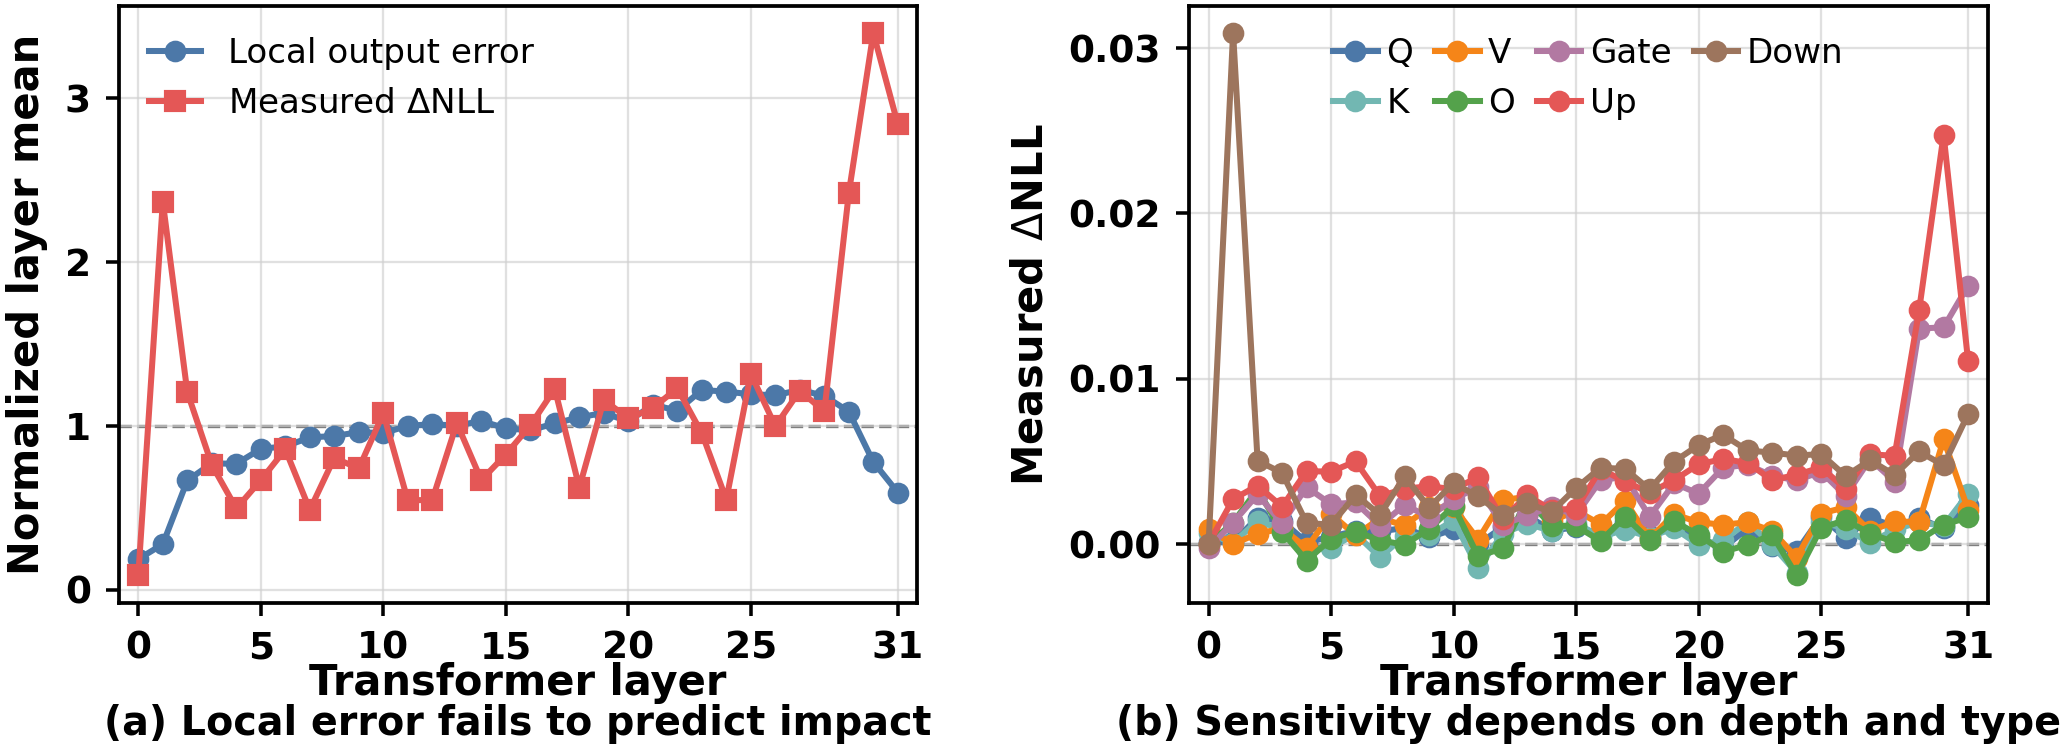
\includegraphics[width=\columnwidth]{Figures/draft/quality.png}
    \caption{Illustration of the structure-dependent relationship between local output perturbations and global quality degradation. The final figure may compare depth buckets, module types, or local error against measured $\Delta\mathrm{NLL}$.}
    \label{fig:quality-sensitivity}
    \vspace{-6pt}
\end{figure}

We therefore introduce a structure-aware local-to-global calibration that aggregates local errors according to compression method, depth bucket, and module type. For inference phase $r\in\{p,d\}$, we define
\begin{equation}
X_{c,b,t}^{r}(\pi)
=
\sum_{\substack{
i:\,a_i^{r}=c,\\
b(i)=b,\,t(i)=t
}}
e_{i,c},
\end{equation}
where $a_i^{r}$ denotes the compression method selected for module $v_i$ in phase $r$, while $b(i)$ and $t(i)$ denote its depth bucket and module type, respectively. For deployment scenario $s=(B,S,T)$, the local perturbations from the two inference phases are combined as
\begin{equation}
X_{c,b,t}(\pi;s)
=
X_{c,b,t}^{p}(\pi)
+
T\,X_{c,b,t}^{d}(\pi),
\end{equation}
where $T$ is the target generation length and reflects the accumulated effect of decoding-time compression over successive generation steps.

To learn structural sensitivity from a limited number of policy-level NLL measurements, we avoid assigning an independent parameter to every module or every $(c,b,t)$ combination. Instead, we use a factorized parameterization
\begin{equation}
w_{c,b,t}
=
\operatorname{softplus}
\left(
g+u_c+v_b+z_t
\right),
\end{equation}
where $g$ is a shared base sensitivity, $u_c$, $v_b$, and $z_t$ capture the sensitivity variations associated with the compression method, depth bucket, and module type, respectively, and $\operatorname{softplus}(x)=\log(1+e^x)$ ensures nonnegative weights. This factorization allows modules with shared structural attributes to share statistical strength, capturing the dominant sources of quality variation with relatively few parameters. The nonnegativity constraint prevents negative coefficients from canceling local errors, which could otherwise produce unrealistically small estimates of quality degradation.

The predicted quality degradation of policy $\pi$ is finally given by
\begin{equation}
\widehat{\Delta Q}(\pi;s)
=
\beta
+
\sum_{c,b,t}
\widetilde{X}_{c,b,t}(\pi;s)
w_{c,b,t},
\end{equation}
where $\widetilde{X}_{c,b,t}$ denotes the normalized aggregated error and $\beta$ is a global bias term. The parameters are calibrated using the measured $\Delta\mathrm{NLL}$ values of a small set of representative heterogeneous policies.

\subsection{Strategy Optimization and Deployment}

With the latency and quality models established, the abstract problem in Eq.~(\ref{eq:problem}) reduces to a concrete instance: each legal action $a\in\mathcal{A}_i$ is now associated with latency and quality costs $\ell_{i,a}$ and $q_{i,a}$. Given the quality budget $\epsilon$, we introduce a binary variable $x_{i,a}$ for each module--action pair, with the constraint $\sum_{a\in\mathcal{A}_i}x_{i,a}=1$ ensuring exactly one action per module. The compression strategy is obtained by solving the multiple-choice knapsack problem
\begin{equation}
\begin{aligned}
\min_{\{x_{i,a}\}}\quad
& \sum_{i=1}^{M}\sum_{a\in\mathcal{A}_i}
x_{i,a}\ell_{i,a}
\quad
\mathrm{s.t.}\quad
\sum_{i=1}^{M}\sum_{a\in\mathcal{A}_i}
x_{i,a}q_{i,a}\leq \epsilon.
\end{aligned}
\end{equation}

To solve the problem, we discretize the quality cost into $K$ bins and use dynamic programming to maintain the minimum latency attainable under different cumulative quality budgets while processing the modules sequentially. States that are no better in either quality cost or latency than another state are removed. The time complexity is $O(K\sum_{i=1}^{M}|\mathcal{A}_i|)$ with $O(K)$ working memory. For Llama-2-7B, the optimization requires approximately XX seconds.



Furthermore, we integrate our heterogeneous compression policies into vLLM for practical deployment. The main overhead comes from switching compressed representations between stages; we hide this by materializing decoding weights on a dedicated copy stream while prefill proceeds on subsequent layers, overlapping weight switching with computation.

% For deployment, the optimized policy is executed through an extended vLLM runtime. \textbf{TODO:} describe policy representation and loading, backend routing between prefill and decoding, compressed-weight materialization and caching, and heterogeneous kernel optimizations.



% Revised experimental section for an AAAI-style two-column paper.
% Suggested packages:
% \usepackage{booktabs}
% \usepackage{multirow}
% \usepackage{graphicx}

\section{Experiments}
\begin{table*}[t]
\centering
\caption{Quality and speedup on the RTX~5090 and RTX~PRO~6000. TTFT, TPOT, and E2E speedups are measured relative to BF16 on the same GPU.}
\label{tab:overall_results}
\setlength{\tabcolsep}{2.2pt}
\resizebox{\textwidth}{!}{
\begin{tabular}{llccccc|cccccc}
\toprule
& &
\multicolumn{5}{c}{\textbf{Prefill-only}} &
\multicolumn{6}{c}{\textbf{Prefill--Decode}} \\
Model & Method &
ARC-C & ARC-E & Wino. & MMLU & TTFT &
CNN/DM & DialogSum & IWSLT'17 & TTFT & TPOT & E2E \\
& &
Acc. & Acc. & Acc. & Acc. & $\times$ &
R-L & R-L & BLEU & $\times$ & $\times$ & $\times$ \\
\midrule
\multicolumn{13}{l}{\textbf{(a) NVIDIA RTX 5090}} \\
\midrule
\multirow{7}{*}{\shortstack[c]{Llama-2\\7B-Chat}}
& BF16                & 43.34 & 72.81 & 68.27 & 46.57 & 1.00 & 23.67 & 21.69 & 19.30 & 1.00 & 1.00 & 1.00 \\
& Dense NVFP4         & 43.17 & 71.13 & 67.80 & 44.94 & 1.71 & 24.27 & 20.59 & 16.84 & 1.64 & 0.55 & 0.80 \\
& Sparse BF16         & 35.07 & 63.85 & 63.85 & 28.24 & 1.53 & 15.35 & 13.54 &  3.90 & 1.56 & 0.91 & 1.13 \\
& Sparse NVFP4        & 23.38 & 36.62 & 50.43 & 23.09 & 1.86 & 15.96 & 13.57 &  1.57 & 1.62 & 0.52 & 0.77 \\
& W4A16 Marlin        & 43.09 & 71.89 & 68.82 & 45.66 & 1.02 & 23.73 & 21.77 & 18.85 & 0.97 & 1.50 & 1.19 \\
& Ours (Max speed)    & 27.73 & 53.16 & 56.75 & 23.51 & 2.08 & 18.56 & 13.57 &  2.60 & 1.50 & 1.60 & 1.55 \\
& Ours (Balanced)     & 43.69 & 70.58 & 67.32 & 44.35 & 1.74 & 23.80 & 21.40 & 21.08 & 1.03 & 1.26 & 1.14 \\
\midrule
\multirow{7}{*}{\shortstack[c]{Llama-3.1\\8B-Instruct}}
& BF16                & 55.63 & 81.99 & 73.48 & 68.40 & 1.00 & 19.39 & 13.48 & 10.78 & 1.00 & 1.00 & 1.00 \\
& Dense NVFP4         & 51.11 & 79.29 & 72.06 & 63.50 & 1.76 & 17.11 &  9.54 & 10.51 & 1.71 & 0.53 & 0.83 \\
& Sparse BF16         & 38.74 & 68.18 & 66.06 & 42.96 & 1.54 &  6.76 &  5.11 &  3.04 & 1.53 & 0.88 & 1.13 \\
& Sparse NVFP4        & 26.37 & 45.66 & 53.28 & 23.88 & 1.93 &  4.25 &  0.41 &  0.05 & 1.81 & 0.49 & 0.79 \\
& W4A16 Marlin        & 53.67 & 80.93 & 73.09 & 66.20 & 0.98 & 17.50 &  9.75 & 10.56 & 0.98 & 1.27 & 1.10 \\
& Ours (Max speed)    & 33.02 & 61.28 & 61.09 & 31.14 & 2.26 & 14.59 &  4.21 &  1.29 & 1.74 & 1.18 & 1.42 \\
& Ours (Balanced)     & 49.23 & 77.82 & 70.64 & 55.93 & 1.91 & 18.84 & 11.48 & 10.55 & 1.40 & 1.13 & 1.26 \\
\midrule
\multicolumn{13}{l}{\textbf{(b) NVIDIA RTX PRO 6000}} \\
\midrule
\multirow{7}{*}{\shortstack[c]{Llama-2\\7B-Chat}}
& BF16                & -- & -- & -- & -- & 1.00 & -- & -- & -- & 1.00 & 1.00 & 1.00 \\
& Dense NVFP4         & -- & -- & -- & -- & --   & -- & -- & -- & --   & --   & -- \\
& Sparse BF16         & -- & -- & -- & -- & --   & -- & -- & -- & --   & --   & -- \\
& Sparse NVFP4        & -- & -- & -- & -- & --   & -- & -- & -- & --   & --   & -- \\
& W4A16 Marlin        & -- & -- & -- & -- & --   & -- & -- & -- & --   & --   & -- \\
& Ours ($\epsilon_1$) & -- & -- & -- & -- & --   & -- & -- & -- & --   & --   & -- \\
& Ours ($\epsilon_2$) & -- & -- & -- & -- & --   & -- & -- & -- & --   & --   & -- \\
\midrule
\multirow{7}{*}{\shortstack[c]{Llama-3.1\\8B-Instruct}}
& BF16                & -- & -- & -- & -- & 1.00 & -- & -- & -- & 1.00 & 1.00 & 1.00 \\
& Dense NVFP4         & -- & -- & -- & -- & --   & -- & -- & -- & --   & --   & -- \\
& Sparse BF16         & -- & -- & -- & -- & --   & -- & -- & -- & --   & --   & -- \\
& Sparse NVFP4        & -- & -- & -- & -- & --   & -- & -- & -- & --   & --   & -- \\
& W4A16 Marlin        & -- & -- & -- & -- & --   & -- & -- & -- & --   & --   & -- \\
& Ours ($\epsilon_1$) & -- & -- & -- & -- & --   & -- & -- & -- & --   & --   & -- \\
& Ours ($\epsilon_2$) & -- & -- & -- & -- & --   & -- & -- & -- & --   & --   & -- \\
\bottomrule
\end{tabular}}
\end{table*}
\subsection{Experimental Setup}

\paragraph{Models, workloads, and metrics.}
We evaluate our framework on Llama-2-7B-Chat and Llama-3.1-8B-Instruct under two representative workloads. The \emph{prefill-only} workload uses $B=8$ and $S=2048$, while the \emph{prefill--decoding} workload uses $B=16$, $S=2048$, and $T=80$. For prefill-only evaluation, we report accuracy on ARC-Challenge, ARC-Easy, WinoGrande, and MMLU~\cite{clark2018arc,sakaguchi2020winogrande,hendrycks2021mmlu}. Following FlexQuant~\cite{liu2025flexquant}, generation quality is evaluated on CNN/DailyMail, DialogSum, and IWSLT~2017~\cite{nallapati2016cnndm,chen2021dialogsum,cettolo2017iwslt} under the prefill--decoding workload, using ROUGE-L~\cite{lin2004rouge} for summarization and BLEU~\cite{papineni2002bleu} for translation. End-to-end performance is reported as speedup over the BF16 model under the same hardware and workload.

\paragraph{Baselines.}
We compare against five uniform model-wide configurations: the uncompressed BF16 model, dense NVFP4~\cite{alvarez2025nvfp4} quantized with round-to-nearest, sparse BF16 produced by SparseGPT~\cite{frantar2023sparsegpt} with WikiText-2 calibration~\cite{merity2017wikitext}, sparse NVFP4 obtained by further quantizing the SparseGPT model, and W4A16 executed with the Marlin kernel~\cite{frantar2025marlin}. Each baseline applies one configuration uniformly to all supported modules and both inference stages. Our method selects module- and stage-specific actions from the same candidate pool, with BF16 retained as a legal fallback.

\paragraph{Hardware and implementation.}
Experiments are conducted on NVIDIA RTX~5090 and RTX~PRO~6000 Blackwell GPUs. We integrate our framework into vLLM~0.11.1~\cite{kwon2023vllm}. Dense and sparse NVFP4 kernels are implemented with CUTLASS, sparse BF16 uses cuSPARSELt, and W4A16 uses the Marlin implementation in vLLM. Compressed weights are materialized before inference and reused across requests. Each latency result is averaged over \textbf{[R]} runs after \textbf{[W]} warm-up runs. Because the optimizer produces hardware-specific strategies, quality and latency are evaluated separately on each GPU. The latency model uses \textbf{[N$_L$]} kernel measurements and \textbf{[N$_P$]} complete policies, while the quality model is calibrated with \textbf{[N$_Q$]} sequences and \textbf{[N$_S$]} sampled policies.

\subsection{Overall Results}



\paragraph{End-to-end comparison.}
Table~\ref{tab:overall_results} compares our hardware-specific heterogeneous strategies with uniform compression baselines. Under the stricter quality budget $\epsilon_1$, our method limits the quality degradation to \textbf{[X]} while achieving up to \textbf{[Y$\times$]} speedup on the RTX~5090 and \textbf{[Z$\times$]} on the RTX~PRO~6000. Relaxing the budget to $\epsilon_2$ further improves performance to \textbf{[Y$_2\times$]} and \textbf{[Z$_2\times$]}, respectively. At comparable quality, our method consistently outperforms the best uniform configuration across both models and workloads, demonstrating the benefit of adapting compression choices to module shapes, inference stages, and target hardware.

\begin{figure}[t]
\centering
\begin{minipage}[t]{0.48\linewidth}
\centering
\fbox{\parbox[c][2.8cm][c]{0.94\linewidth}{
\centering
\textbf{Llama-2-7B-Chat}\\
Trade-off placeholder
}}
\end{minipage}
\hfill
\begin{minipage}[t]{0.48\linewidth}
\centering
\fbox{\parbox[c][2.8cm][c]{0.94\linewidth}{
\centering
\textbf{Llama-3.1-8B-Instruct}\\
Trade-off placeholder
}}
\end{minipage}
\caption{Measured latency--quality trade-offs under the prefill--decoding workload. Each panel shows uniform baselines, strategies returned under different quality budgets, and the empirical frontier obtained from \textbf{[N]} measured policies. Our strategies remain within \textbf{[X\%]} of the empirical frontier while requiring only \textbf{[Y\%]} of the evaluation cost. We use prefill--decoding because it covers both inference stages and is therefore the most representative setting for stage-wise optimization.}
\label{fig:pareto_tradeoff}
\end{figure}

\paragraph{Trade-off quality.}
Figure~\ref{fig:pareto_tradeoff} varies the quality budget and compares the resulting strategies with a large-scale measured search. The selected strategies closely track the empirical Pareto frontier, with an average latency gap of \textbf{[X\%]} at matched quality. Constructing the reference frontier requires \textbf{[C]} GPU-hours, whereas our framework relies only on the limited profiling and calibration data described above.

\subsection{Ablation Studies}

\begin{figure}[t]
\centering
\fbox{\parbox[c][2.9cm][c]{0.94\linewidth}{
\centering
\textbf{(a) Latency prediction and ablation}\\
Predicted vs.\ measured latency for:\\
Roofline $\rightarrow$ shape correction $\rightarrow$ policy calibration
}}
\vspace{1mm}

\fbox{\parbox[c][2.9cm][c]{0.94\linewidth}{
\centering
\textbf{(b) Quality prediction and ablation}\\
Predicted vs.\ measured $\Delta$NLL for:\\
local-error sum $\rightarrow$ structure-aware weighting $\rightarrow$ factorized model
}}
\vspace{1mm}

\fbox{\parbox[c][2.4cm][c]{0.94\linewidth}{
\centering
\textbf{(c) Calibration sample efficiency}\\
Prediction error and selected-policy performance versus the number of calibration policies
}}
\caption{Prediction accuracy and ablation of the latency and quality models. Each prediction plot progressively adds the proposed modeling components, directly showing how the estimates approach the measured values. Panel (c) studies the effect of policy-level calibration set size.}
\label{fig:modeling_ablation}
\end{figure}

\paragraph{Latency-model ablation.}
Figure~\ref{fig:modeling_ablation}(a) shows that the method-aware Roofline baseline captures the global performance trend but remains inaccurate for irregular and small-$m$ shapes. Adding shape-dependent correction reduces the prediction error from \textbf{[X\%]} to \textbf{[Y\%]}, while policy-level calibration further improves the end-to-end MAPE to \textbf{[Z\%]} and the Spearman correlation to \textbf{[R]}.

\paragraph{Quality-model ablation.}
As shown in Fig.~\ref{fig:modeling_ablation}(b), directly summing module-level errors provides only a coarse estimate of strategy quality. Structure-aware weighting substantially improves strategy ranking by accounting for module type and depth, and the factorized nonnegative model achieves the lowest held-out MAE of \textbf{[X]} and a Spearman correlation of \textbf{[Y]}.

\paragraph{Calibration sample efficiency.}
Figure~\ref{fig:modeling_ablation}(c) varies the number of complete strategies used for calibration. Prediction error decreases rapidly with the first \textbf{[N$_0$]} strategies and stabilizes after approximately \textbf{[N$_1$]}. The final strategy selected with this reduced calibration set remains within \textbf{[X\%]} latency and \textbf{[Y]} quality loss of the strategy obtained using the full set.

\begin{table}[t]
\centering
\caption{Runtime ablation under the prefill--decoding workload. This table may be omitted if space is limited.}
\label{tab:runtime_ablation}
\setlength{\tabcolsep}{4pt}
\begin{tabular}{lcc}
\toprule
Runtime configuration & E2E latency & Overhead \\
\midrule
Naive heterogeneous dispatch & -- & -- \\
$+$ stage-aware routing       & -- & -- \\
$+$ compressed-weight caching & -- & -- \\
\bottomrule
\end{tabular}
\end{table}

\paragraph{Runtime integration.}
Table~\ref{tab:runtime_ablation} isolates the runtime components required to execute heterogeneous strategies efficiently. Stage-aware routing enables different kernels to be used in prefill and decoding, while compressed-weight caching avoids repeated format conversion. Together, they reduce runtime overhead from \textbf{[X\%]} to \textbf{[Y\%]} and preserve most of the acceleration predicted by the optimizer.







% \section{Experiments}

% \subsection{Experimental Setup}

% \paragraph{Baselines.}
% % TODO.

% \paragraph{Models and Datasets.}
% % TODO.

% \paragraph{Deployment Scenarios and Hardware.}
% % TODO.

% \paragraph{Implementation Details.}
% % TODO.

% \subsection{Overall Results}


% \begin{table*}[t]
% \centering
% \caption{
% Overall comparison with uniform compression baselines.
% Speedup is measured against dense BF16.
% For prefill-only, quality is measured by ARC-Challenge accuracy.
% For prefill-decoding, we report ROUGE-L on CNN/DailyMail and DialogSum,
% and BLEU on IWSLT2017.
% }
% \label{tab:overall_results}

% \resizebox{\textwidth}{!}{
% \begin{tabular}{ll|cc|cccc}
% \toprule

% Model & Method
% &
% \multicolumn{2}{c|}{Prefill-only}
% &
% \multicolumn{4}{c}{Prefill-Decoding}
% \\

% &
% &
% Speedup $\uparrow$
% &
% ARC Acc. $\uparrow$
% &
% Speedup $\uparrow$
% &
% CNN/DM R-L $\uparrow$
% &
% DialogSum R-L $\uparrow$
% &
% IWSLT BLEU $\uparrow$
% \\

% \midrule

% \multirow{7}{*}{\centering Llama-2-7B-Chat}

% &Dense BF16
% &1.00&43.345
% &1.00&23.671&21.688&19.296
% \\

% &Dense NVFP4
% &1.87&42.833
% &1.19&24.273&20.592&16.835
% \\

% &Sparse BF16
% &1.63&35.324
% &1.44&15.350&13.539&3.900
% \\

% &Sparse NVFP4
% &2.07&23.976
% &1.19&2.047&9.388&0.238
% \\

% &Marlin NVFP4
% &1.04&42.833
% &1.39&24.579&21.368&18.200
% \\

% \cmidrule{2-8}

% &Ours (High-quality)
% &1.73&44.198
% &1.68&23.754&21.633&19.029
% \\

% &Ours (High-speed)
% &2.04&28.072
% &1.71&23.544&21.581&18.301
% \\


% \midrule


% \multirow{7}{*}{\centering Llama-3.1-8B-Instruct}

% &Dense BF16
% &1.00&55.375
% &1.00&19.487&13.784&10.680
% \\

% &Dense NVFP4
% &1.73&54.096
% &1.06&16.345&8.203&10.312
% \\

% &Sparse BF16
% &1.55&38.737
% &1.17&12.834&4.049&3.276
% \\

% &Sparse NVFP4
% &1.92&26.792
% &0.79&0.804&0.126&0.014
% \\

% &Marlin NVFP4
% &1.03&54.096
% &1.16&16.108&8.805&10.403
% \\

% \cmidrule{2-8}

% &Ours (High-quality)
% &1.56&54.863
% &1.48&16.675&11.122&10.582
% \\

% &Ours (High-speed)
% &2.17&33.106
% &1.69&16.840&9.085&10.570
% \\

% \bottomrule
% \end{tabular}
% }
% \end{table*}



% % TODO:
% % 1. Comprehensive quality and speed table.
% % 2. Speed--quality Pareto frontier.
% % 3. Optimization overhead.

% \subsection{Ablation Studies}

% TODO:
% 1. Quality-prediction accuracy and ablations.
% 2. Latency-prediction accuracy and ablations.
% 3. vLLM integration/runtime ablations.

\section{Conclusion}


\bibliography{aaai2027}

% Check whether the conference requires a reproducibility checklist to be included in the paper.
% If so, you can uncomment the following line and ajust the path to include it.
% \input{ReproducibilityChecklist.tex}

\end{document}
